\documentclass[]{article}
\usepackage{graphicx}

%opening
\title{CPSC425 A1}
\author{Eric Semeniuc - 54383161}

\begin{document}

\maketitle


\textbf{1-1:}
\begin{verbatim}

>>> main.boxfilter(3)
array([[0.11111111, 0.11111111, 0.11111111],
[0.11111111, 0.11111111, 0.11111111],
[0.11111111, 0.11111111, 0.11111111]])
>>> main.boxfilter(4)

Traceback (most recent call last):
File "<input>", line 1, in <module>
main.boxfilter(4)
File "/home/eric/cs425/a1/main.py", line 12, in boxfilter
assert isOdd(n)
AssertionError
>>> main.boxfilter(5)

array([[0.04, 0.04, 0.04, 0.04, 0.04],
[0.04, 0.04, 0.04, 0.04, 0.04],
[0.04, 0.04, 0.04, 0.04, 0.04],
[0.04, 0.04, 0.04, 0.04, 0.04],
[0.04, 0.04, 0.04, 0.04, 0.04]])
>>> 
\end{verbatim}


\textbf{1-2:}
\begin{verbatim}
>>> main.gauss1d(0.3)
array([0.00383626, 0.99232748, 0.00383626])
>>> main.gauss1d(0.5)
array([0.10650698, 0.78698604, 0.10650698])
>>> main.gauss1d(1)
array([0.00443305, 0.05400558, 0.24203623, 0.39905028, 0.24203623,
0.05400558, 0.00443305])
>>> main.gauss1d(2)
array([0.0022182 , 0.00877313, 0.02702316, 0.06482519, 0.12110939,
0.17621312, 0.19967563, 0.17621312, 0.12110939, 0.06482519,
0.02702316, 0.00877313, 0.0022182 ])
>>> 
\end{verbatim}


\textbf{1-3:}
\begin{verbatim}
>>> main.gauss2d(0.5)
array([[0.01134374, 0.08381951, 0.01134374],
[0.08381951, 0.61934703, 0.08381951],
[0.01134374, 0.08381951, 0.01134374]])
>>> main.gauss2d(1)
array([[1.96519161e-05, 2.39409349e-04, 1.07295826e-03, 1.76900911e-03,
1.07295826e-03, 2.39409349e-04, 1.96519161e-05],
[2.39409349e-04, 2.91660295e-03, 1.30713076e-02, 2.15509428e-02,
1.30713076e-02, 2.91660295e-03, 2.39409349e-04],
[1.07295826e-03, 1.30713076e-02, 5.85815363e-02, 9.65846250e-02,
5.85815363e-02, 1.30713076e-02, 1.07295826e-03],
[1.76900911e-03, 2.15509428e-02, 9.65846250e-02, 1.59241126e-01,
9.65846250e-02, 2.15509428e-02, 1.76900911e-03],
[1.07295826e-03, 1.30713076e-02, 5.85815363e-02, 9.65846250e-02,
5.85815363e-02, 1.30713076e-02, 1.07295826e-03],
[2.39409349e-04, 2.91660295e-03, 1.30713076e-02, 2.15509428e-02,
1.30713076e-02, 2.91660295e-03, 2.39409349e-04],
[1.96519161e-05, 2.39409349e-04, 1.07295826e-03, 1.76900911e-03,
1.07295826e-03, 2.39409349e-04, 1.96519161e-05]])
>>> 
\end{verbatim}

\textbf{1-4}
Scipy has has a separate convolve2d and correlate2d for situations when the the filter is not a 180 rotation of itself
\begin{figure}[H]
	\centering
	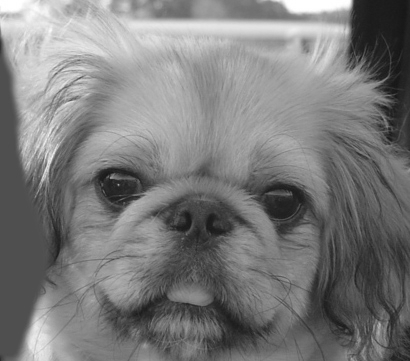
\includegraphics{dog-grey.png}
	\label{fig:dog-grey}
\end{figure}

\begin{figure}[H]
	\centering
	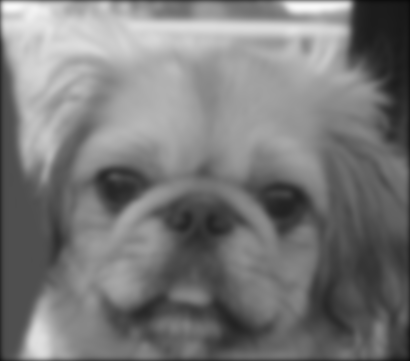
\includegraphics{dog-greyblur.png}
	\label{fig:dog-grey-blur}
\end{figure}

\textbf{1-5}

2d convolution is separable, so we can separate the 2d filter into to column vectors instead.
To use the 2 column vectors, we apply a 1d convolution along the rows on the image with the first vector, 
then do a second pass of 1d convolution on the columns with the second vector. The runtime would be $O(n^2 * m)$
rather than $O(n^2 * m^2)$


\textbf{2-3}
\begin{figure}[H]
	\centering
	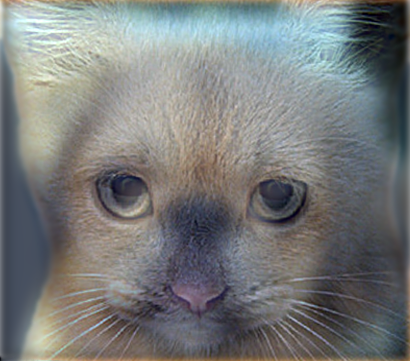
\includegraphics{catdog.png}
	\label{fig:catdog}
\end{figure}

\begin{figure}[H]
	\centering
	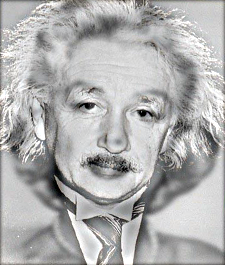
\includegraphics{meinstein.png}
	\label{fig:meinstein}
\end{figure}

\begin{figure}[H]
	\centering
	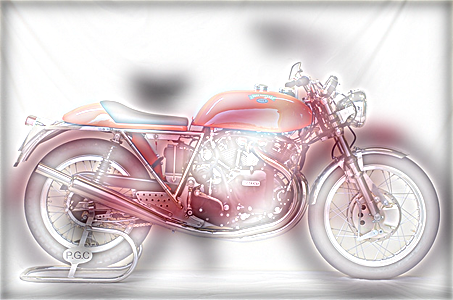
\includegraphics{bike-moto.png}
	\label{fig:bike-moto}
\end{figure}
\end{document}
